\section{Alloy}
\lstset{
  language=alloy,
  basicstyle=\small\ttfamily,
  breaklines=true,
  showstringspaces=false
}
In this section it is provided a representation of the world of CKB using the Alloy language. Every run and every check are commented in order to guarantee a syntactical correct compilation of the code: it is up to the reader to decide what to uncomment based on their will.

\lstinputlisting{4Alloy/res/third_model.als}

\subsection{Generated Worlds}
\begin{figure}[h]
  \centering
  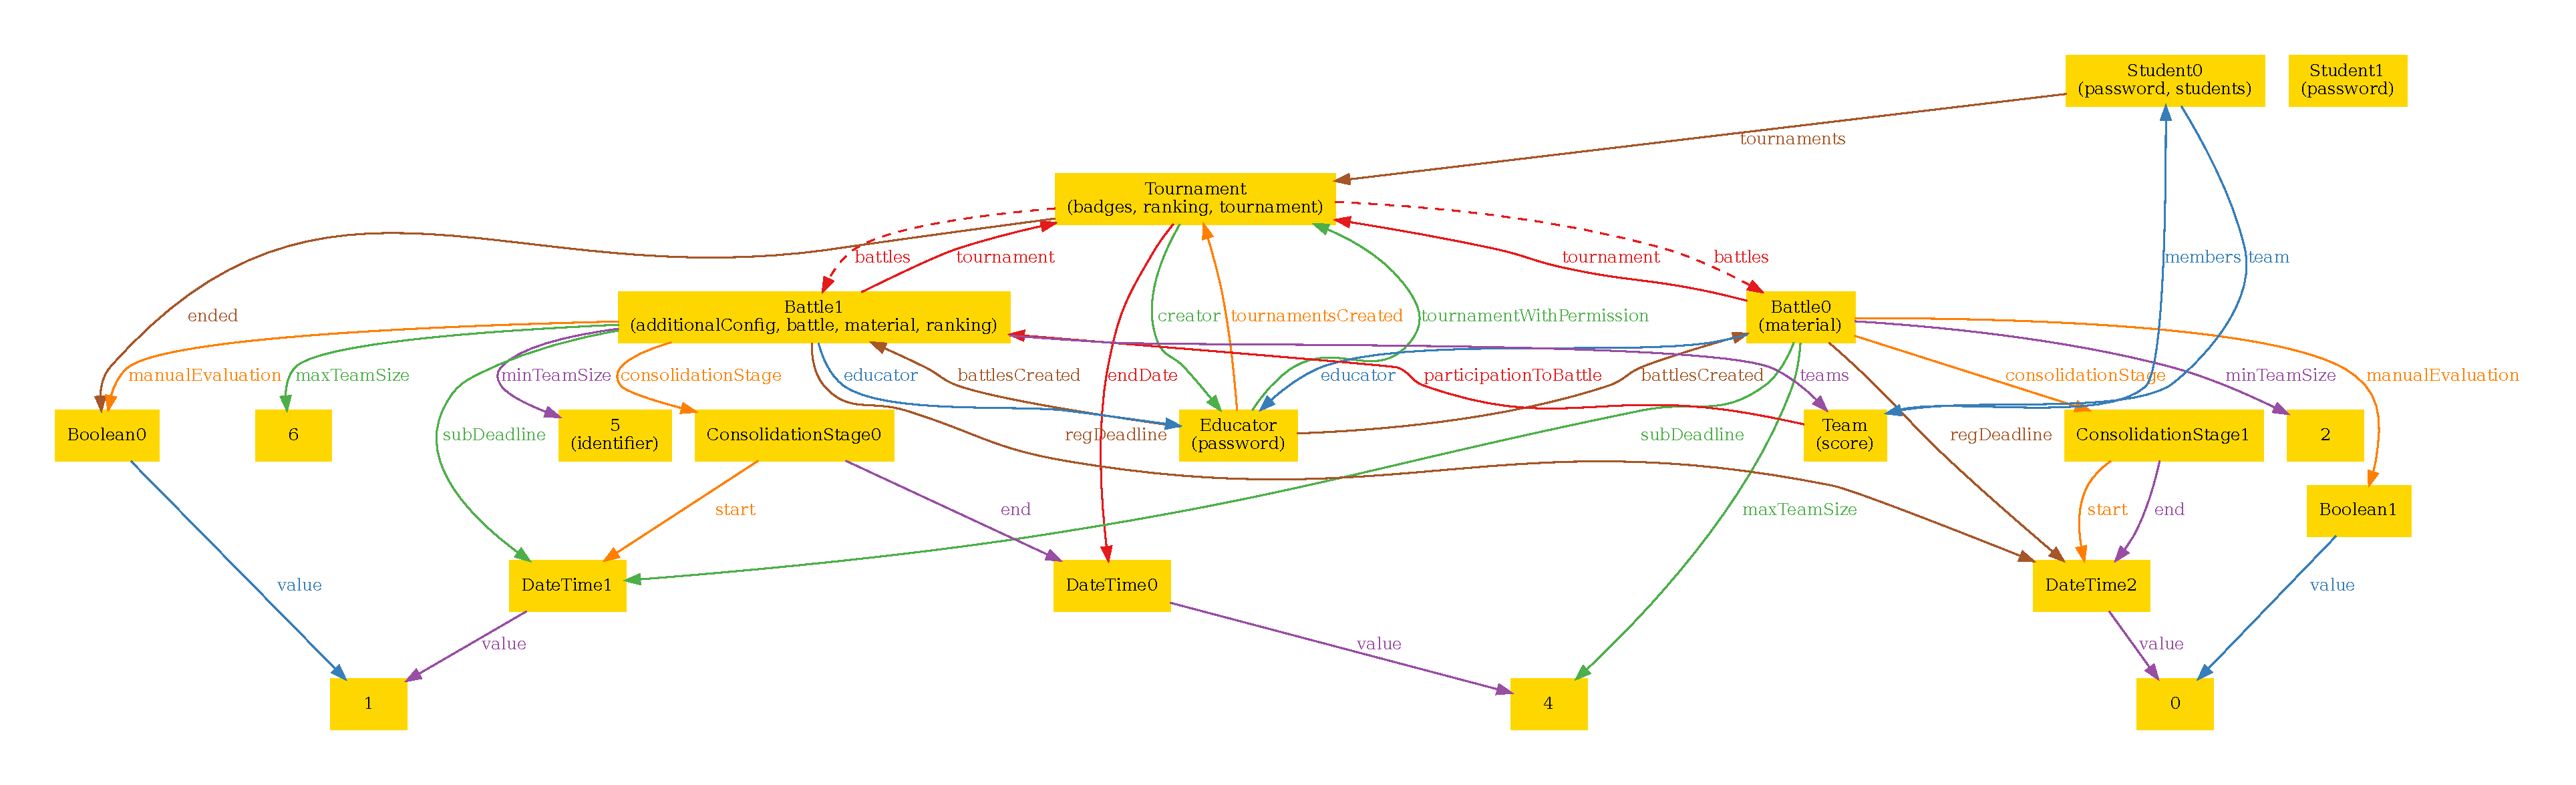
\includegraphics[width=1\linewidth]{RASD/4Alloy/res/noManualEvaluation.pdf}
  \caption{The figure shows generated by running \textit{noManualEvaluation} predicate projected over thirteen signatures (ABS, Badge, CodeTest, Description, EducatorMaterial, EvaluationCriteria, GitHubName, GitHubPassword, GitHubRepoLink, Macrovariables, Notification, Score, String) in order to be more comprehensible. This world represents the situation where there is no manual evaluation for one battle out of two. It is useful in order to see the right aim of the model. Indeed, as you can see, in the case the manualEvaluation is not required (the boolean value equals 0, e.g. for Battle0) there is no consolidation stage, and viceversa (e.g. the case of Battle1). Specifically the world shows the presence of a Tournament consisting of two Battles: a Team made of Student0 (which represents the student himself) is partecipating to Battle1, and so the tournament belongs to his tournaments. The Educator is the creator of the Tournament, so he holds the permissions for it, so why he created Battle0 and Battle1. The tournament is ended, therefore it has a DateTime of the ending. }
\end{figure}

\afterpage{
\begin{figure}[h]
  \centering
  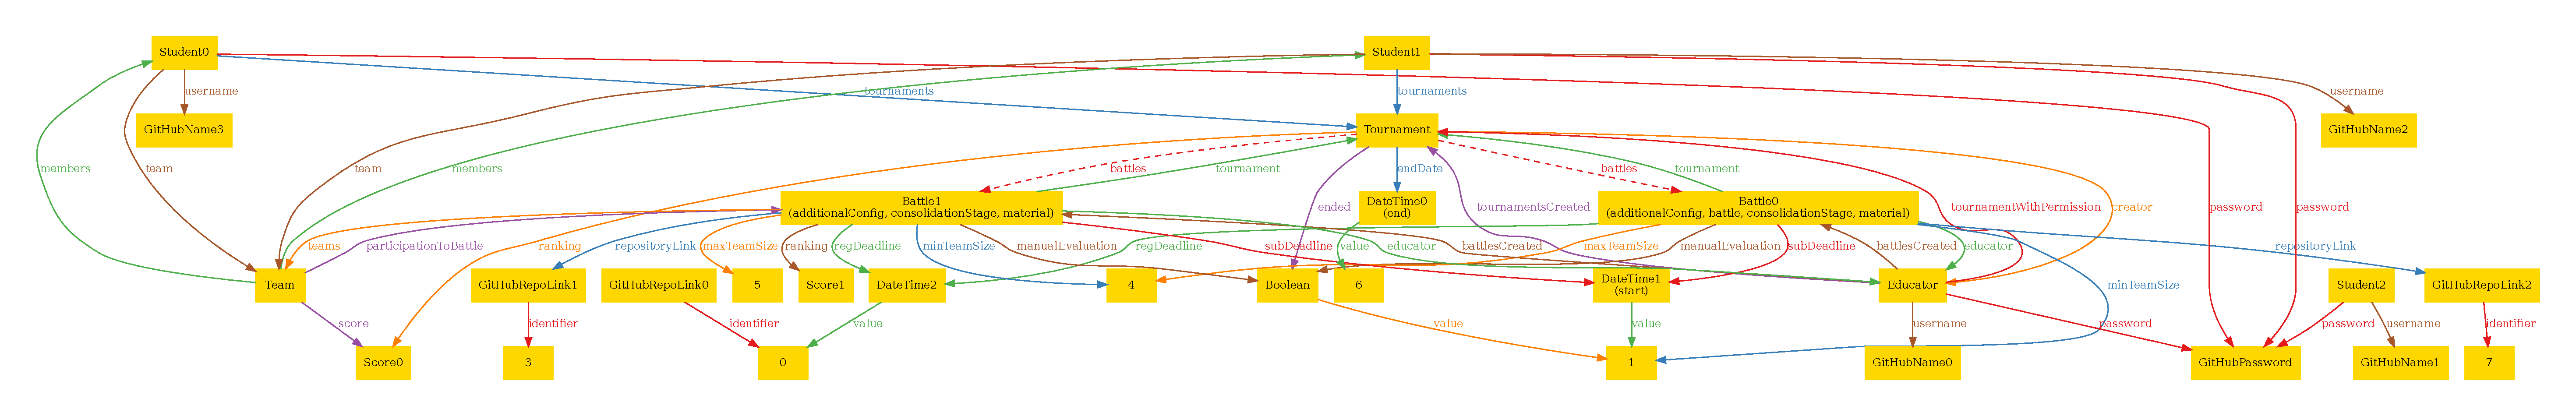
\includegraphics[angle=90, height=1.4\textwidth, width=0.3\textwidth]{RASD/4Alloy/res/general.pdf}
\end{figure}
  \clearpage
  \captionof{figure}{The figure shows world generated by running \textit{general} predicate projected over nine signatures (ABS, CodeTest, ConsolidationStage, Description, EducatorMaterial, EvaluationCriteria, Macrovariables, Notification, String) in order to be more comprehensible. This world represents a normal situation of the model. Specifically it represents the situation where the Student1 is subscribed to a Tournament as the Student0 with whom he participates in Team to the Battle1, created by the Educator, who also created Battle0 and the Tournament itself, and where a Student2 exists without being subscribed to any tournament. Every User has a different GitHubName and a GitHubPassword, and every Battle has a different GitHubRepoLink. Every regDeadline of both the battles has a DateTime value less then the subDeadline one. It is important to notice that where the Tournament has the Educator as its creator, the Educator has this Tournament in its tournaments created and so with his tournaments with permission; furthermore, only Team can participate to Battles, and if a Student member of a Team participate to a Battle in a Tournament, then he has this Tournament inside his tournaments; finally, all the time constraints are respected.}
}

\begin{figure}[h]
\centering
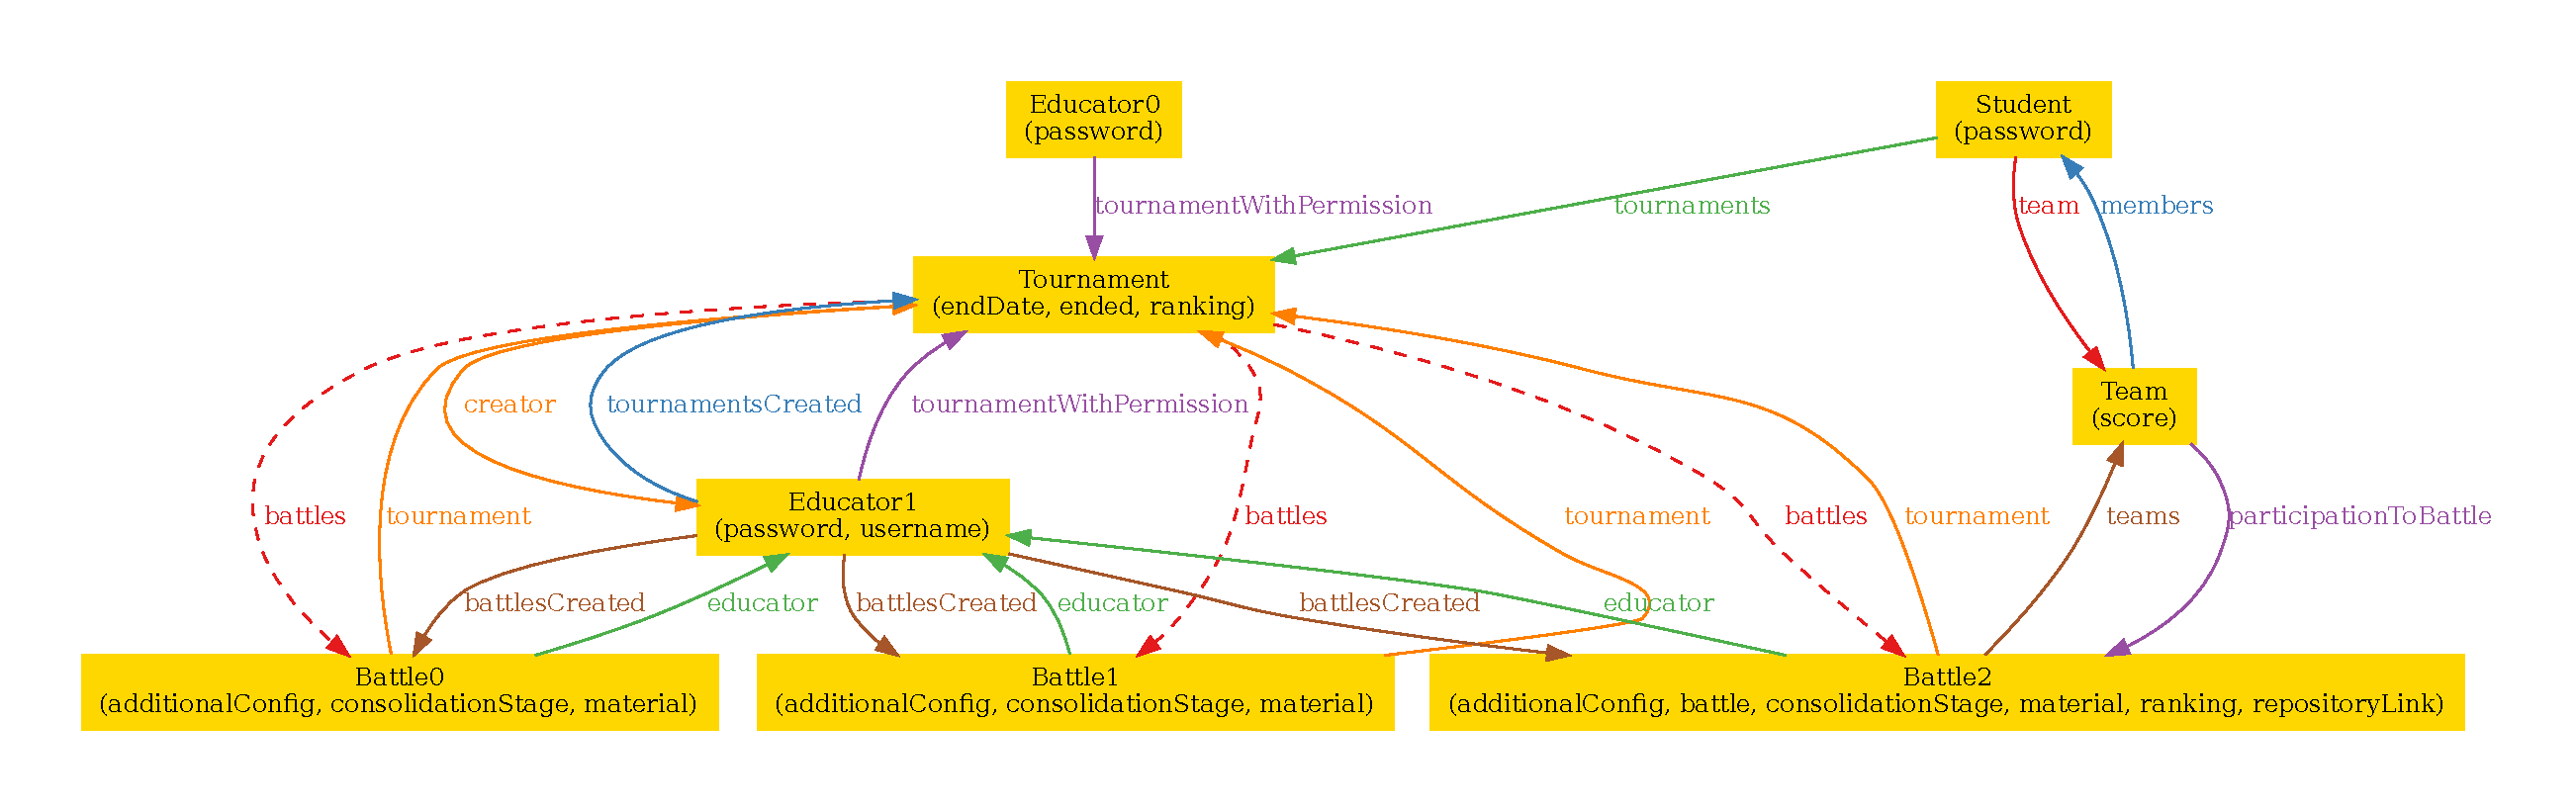
\includegraphics[width=1\linewidth]{RASD/4Alloy/res/educatorsWithOnlyPermission.pdf}
\label{fig:educatorsWithOnlyPermission_alloy}
\caption{The figure shows generated by running \textit{educatorsWithOnlyPermission} projected over seventeen signatures (ABS, Badge, Boolean, CodeTest, ConsolidationStage, DateTime, Description, EducatorMaterial, EvaluationCriteria, GitHubName, GitHubPassword, GitHubRepoLink, Int, Macrovariables, Notification, Score, String) in order to be more comprehensible. This world represents the situation where there are educators with permissions for a tournament they haven't created. As you can see, it cannot exist a tournament without a creator, but some educators can have tournaments with only the permission, without having created them (e.g. Educator0 on Tournament).}
\end{figure}



